% Juego de integración, formato compacto: arquitectura, cuatro resultados
% formales y el demostrador extremo a extremo. Las demostraciones completas de
% los cuatro resultados están en el Anexo~\ref{app:megajuego-full-detail}.
\clearpage
\subsection{Juego de integración}
\label{subsec:megajuego}
\zlabel{budget:megajuego-start}

SP1--SP3 certifican tres interfaces por separado. El juego de integración las
conecta mediante un esquema híbrido sobre continuaciones físicamente
admisibles: cada continuación se admite solo si mejora sobre la política
vigente, sin garantizar el óptimo global del sistema
completo. Una formulación previa de esta misma arquitectura asumía
convergencia al óptimo global; aquí cada bloque certifica solo una mejora
local bajo hipótesis explícitas, y las demostraciones completas están en el
Anexo~\ref{app:megajuego-full-detail}. Su estado aumentado
\begin{equation}
 Y=(X,d,\widehat X,\mathcal E_X,\mathcal I,\Pi^{\mathrm{inc}},\mathcal S,t)
 \label{eq:megajuego-state}
\end{equation}
combina la planta $X$, los compromisos atómicos $d$, la incertidumbre
$\mathcal E_X$, información con procedencia $\mathcal I$ y reservas
espacio--temporales $\mathcal S$ (distintas del catálogo de rutas $\mathcal
R_i^7$ de SP3), para que dos continuaciones se comparen desde el mismo
problema.

\begin{figure}[!htbp]
  \centering
  \begin{tikzpicture}[x=1mm,y=1mm,font=\sffamily\fontsize{7.0}{7.6}\selectfont]
    \tikzset{stage/.style={draw=VIUGray!70,line width=0.5pt,rounded corners=2pt,
        minimum width=42mm,minimum height=17mm,align=center,fill=white},
      arr/.style={-{Latex[length=2.2mm]},line width=0.7pt,draw=VIUDark!70}}
    \node[stage,fill=VIUOrange!8] (est) at (24,10)
      {\textbf{Estado aumentado}\\[1mm]{\fontsize{6.0}{6.5}\selectfont planta, compromisos, incertidumbre}\\
       {\fontsize{6.0}{6.5}\selectfont\color{VIUGray}Ecuación~\eqref{eq:megajuego-state}}};
    \node[stage,fill=SPBlue!8] (cont) at (78,10)
      {\textbf{Continuación causal}\\[1mm]{\fontsize{6.0}{6.5}\selectfont política, contactos, trayectoria predicha}\\
       {\fontsize{6.0}{6.5}\selectfont\color{VIUGray}certifica: mejora sobre la vigente}};
    \node[stage,fill=SPPurple!8] (cert) at (132,10)
      {\textbf{Certificado por bloque}\\[1mm]{\fontsize{6.0}{6.5}\selectfont potencial, KKT, presupuesto}\\
       {\fontsize{6.0}{6.5}\selectfont\color{VIUGray}no certifica: óptimo global del híbrido}};
    \draw[arr] (est.east)--(cont.west);
    \draw[arr] (cont.east)--(cert.west);
  \end{tikzpicture}
  \caption[Arquitectura del juego de integración.]{Arquitectura del juego de
  integración. Cada continuación se admite solo si mejora sobre la política
  vigente y respeta dinámica, contactos, soporte, ruedas, energía, seguridad
  y causalidad informacional simultáneamente; el certificado es válido por
  bloque, no como optimalidad global del sistema híbrido.}
  \label{fig:megajuego-architecture}
  \viuownsource
\end{figure}

\paragraph{Potencial exacto por factores y óptimo central}
Con $\Phi(d,z)=\sum_i\phi_i(z_i)+\sum_a\psi_a(z_{\mathcal I_a})$ y
$J_i=\phi_i+\sum_{a:i\in\mathcal I_a}\psi_a$,

\begin{contribucion}{potencial exacto por factores y certificado de optimalidad central}
\estadoaporte{demostrado; demostraciones completas en el Anexo~\ref{app:megajuego-full-detail}.}
\begin{proposicion}[Potencial exacto por factores]
\label{prop:megajuego-exact-potential}
Si ningún factor omitido de $J_i$ depende de $z_i$, toda desviación unilateral
\emph{admisible} --- la que respeta dinámica, contactos, soporte, ruedas,
energía, seguridad y causalidad informacional de la Figura~\ref{fig:megajuego-architecture} --- cumple $\Delta_iJ_i=\Delta_i\Phi$.
\end{proposicion}
\begin{teorema}[Óptimo central de una rama convexa]
\label{thm:megajuego-central-optimum}
Sean $K$ no vacío, cerrado y convexo, $\Phi$ convexa diferenciable y $F=\operatorname{col}_i\nabla_{z_i}J_i=\nabla\Phi$. Entonces $\langle F(z^\star),z-z^\star\rangle\geq0\ \forall z\in K \iff z^\star\in\arg\min_K\Phi$. Si $\Phi$ es fuertemente convexa, el óptimo primal es único.
\end{teorema}
\end{contribucion}

\paragraph{Separación exacta de trayectorias Bézier cooperativas}
Para dos coaliciones Cargo en discos de radio $1.05$~m con separación
adicional $0.1$~m ($D=2.2$~m),
\begin{equation}
 P_A(s)=(-3+6s,\,a_Ab(s)),\qquad P_B(s)=(3-6s,\,-a_Bb(s)),\qquad b(s)=64s^3(1-s)^3,
 \label{eq:megajuego-bezier-curves}
\end{equation}

\begin{contribucion}{certificado continuo de separación entre trayectorias cooperativas}
\estadoaporte{demostrado algebraicamente; comprobado además con un protocolo de extragradiente en 30 instancias; demostración en el Anexo~\ref{app:megajuego-full-detail}.}
\begin{teorema}[Separación exacta de esta familia]
\label{thm:megajuego-bezier-separation}
Para $0\leq a_A,a_B$ y $0<D\leq\sqrt6$, las trayectorias de la
Ecuación~\eqref{eq:megajuego-bezier-curves} satisfacen $\|P_A(s)-P_B(s)\|\geq D$ para todo $s$ si y solo si $a_A+a_B\geq D$.
\end{teorema}
El óptimo es $a_A^\star=h_BD/(h_A+h_B)$, $a_B^\star=h_AD/(h_A+h_B)$; para pesos
$(h_A,h_B)=(2,1)$, $a_A^\star=11/15$, $a_B^\star=22/15$. El protocolo de
extragradiente alcanzó residual menor que $10^{-9}$ en 113 iteraciones en el
caso principal, y en las 30 instancias de pesos heterogéneos el máximo fue
$9.998\times10^{-10}$ (109--315 iteraciones).
\end{contribucion}

\paragraph{Caging: certificado de contacto con KKT racional}
Para una carga circular de radio $0.45$~m y cuatro contactos cardinales, con
demanda de \emph{wrench} $(20,0,5)$ en N, N y N\,m, el QP
\begin{equation}
 \min_z\tfrac12z^{\mathsf T}z \quad\text{sujeto a}\quad Az=(20,0,5)^{\mathsf T},\ Hz\leq g
 \label{eq:megajuego-caging-qp}
\end{equation}
tiene solución racional exacta de la Ecuación~\eqref{eq:megajuego-caging-qp}
\[
 z^\star=\Big(0,\,0,\,\tfrac{475}{261},\,-\tfrac{190}{261},\,\tfrac{500}{29},\,-\tfrac{200}{29},\,\tfrac{2275}{261},\,-\tfrac{910}{261}\Big),
\]
de valor $513025/2349$ (factibilidad, estacionariedad y multiplicadores no
negativos demostradas algebraicamente en el
Anexo~\ref{app:megajuego-full-detail}), confirmada con SymPy y con un
solucionador numérico independiente del razonamiento algebraico, con brecha
$10^{-11}$.

\paragraph{Presupuesto de ejecución}
\begin{contribucion}{cota de revisiones bajo presupuesto decreciente}
\estadoaporte{demostrado, condicionado a testigo inicial seguro y a presupuesto no negativo; demostración en el Anexo~\ref{app:megajuego-full-detail}.}
\begin{teorema}[Presupuesto de ejecución, condicionado]
\label{thm:megajuego-execution-budget}
Con testigo inicial seguro, tubos que componen, entradas locales realizables y
un presupuesto $W$ que decrece al menos $\kappa_W\Delta t$ durante el
movimiento y en $\delta>0$ por cada sustitución admitida,
$\kappa_WT_{\mathrm{mov}}+\delta N_{\mathrm{rev}}\leq W_0$, donde
$T_{\mathrm{mov}}$ es el tiempo acumulado de movimiento. De ahí
$T_{\mathrm{mov}}\leq W_0/\kappa_W$ y $N_{\mathrm{rev}}\leq\lfloor W_0/\delta\rfloor$.
Tres precisiones delimitan el enunciado. La cota es sobre el tiempo de
movimiento, no sobre la duración de la misión: los intervalos de espera,
deliberación o parada segura no consumen $\kappa_W$ y no están acotados por
este resultado. La finitud de $N_{\mathrm{rev}}$ no requiere suponer ausencia
de Zeno: se sigue de que cada revisión admitida consume $\delta>0$ de un
presupuesto finito, lo que a su vez impide una sucesión infinita de tubos. Y
acotar duración y revisiones no garantiza que se alcance el objetivo, que
puede quedar sin entregar al agotarse el presupuesto.
\end{teorema}
\end{contribucion}

Los cuatro resultados anteriores se demuestran en escenarios concretos y
acotados --- dos coaliciones con una familia geométrica fija de curvas, una
carga circular con cuatro contactos cardinales --- y ninguno certifica que el
sistema híbrido completo, bajo revisiones discretas arbitrarias, alcance un
óptimo global; no generalizan sin nueva demostración a otro número de
coaliciones o de contactos.

\paragraph{Demostrador extremo a extremo}
Un escenario sintético con 15~AMR heterogéneos, 3~cargas (dos Cargo y una
Caging) y 12~robots reclutados ilustra la arquitectura como caso único
determinista, sin repeticiones ni semillas adicionales; no sustituye una
campaña estadística ni una validación de hardware.

\begin{table}[!htbp]
  \centering
  \caption[Escenario extremo a extremo: certificado contra oráculo o cota conocida.]{Escenario
  extremo a extremo: certificado contra oráculo o cota conocida (corrida única, $n=1$, sin réplicas).}
  \label{tab:megajuego-e2e-summary}
  \viutablefont
  \begin{tabularx}{0.92\textwidth}{>{\raggedright\arraybackslash}p{6.2cm} Y}
    \toprule
    Certificado & Resultado \\
    \midrule
    Reclutamiento (subasta distribuida vs.\ oráculo húngaro) & coste $62.83$ en ambos, brecha nula \\
    Orden de coaliciones vs.\ óptimo del catálogo de $3!$ & coincide; $+1.49$\,\% sobre FCFS \\
    Clearance mínimo, entre coaliciones / a obstáculos & $0.655$~m / $0.212$~m \\
    Residual KKT máximo del QP de \emph{caging} & $1.4\times10^{-11}$ \\
    \bottomrule
  \end{tabularx}
  \viusource{elaboración propia, \texttt{simulate\_e2e\_megagame.py}}
\end{table}

\begin{figure}[!htbp]
  \centering
  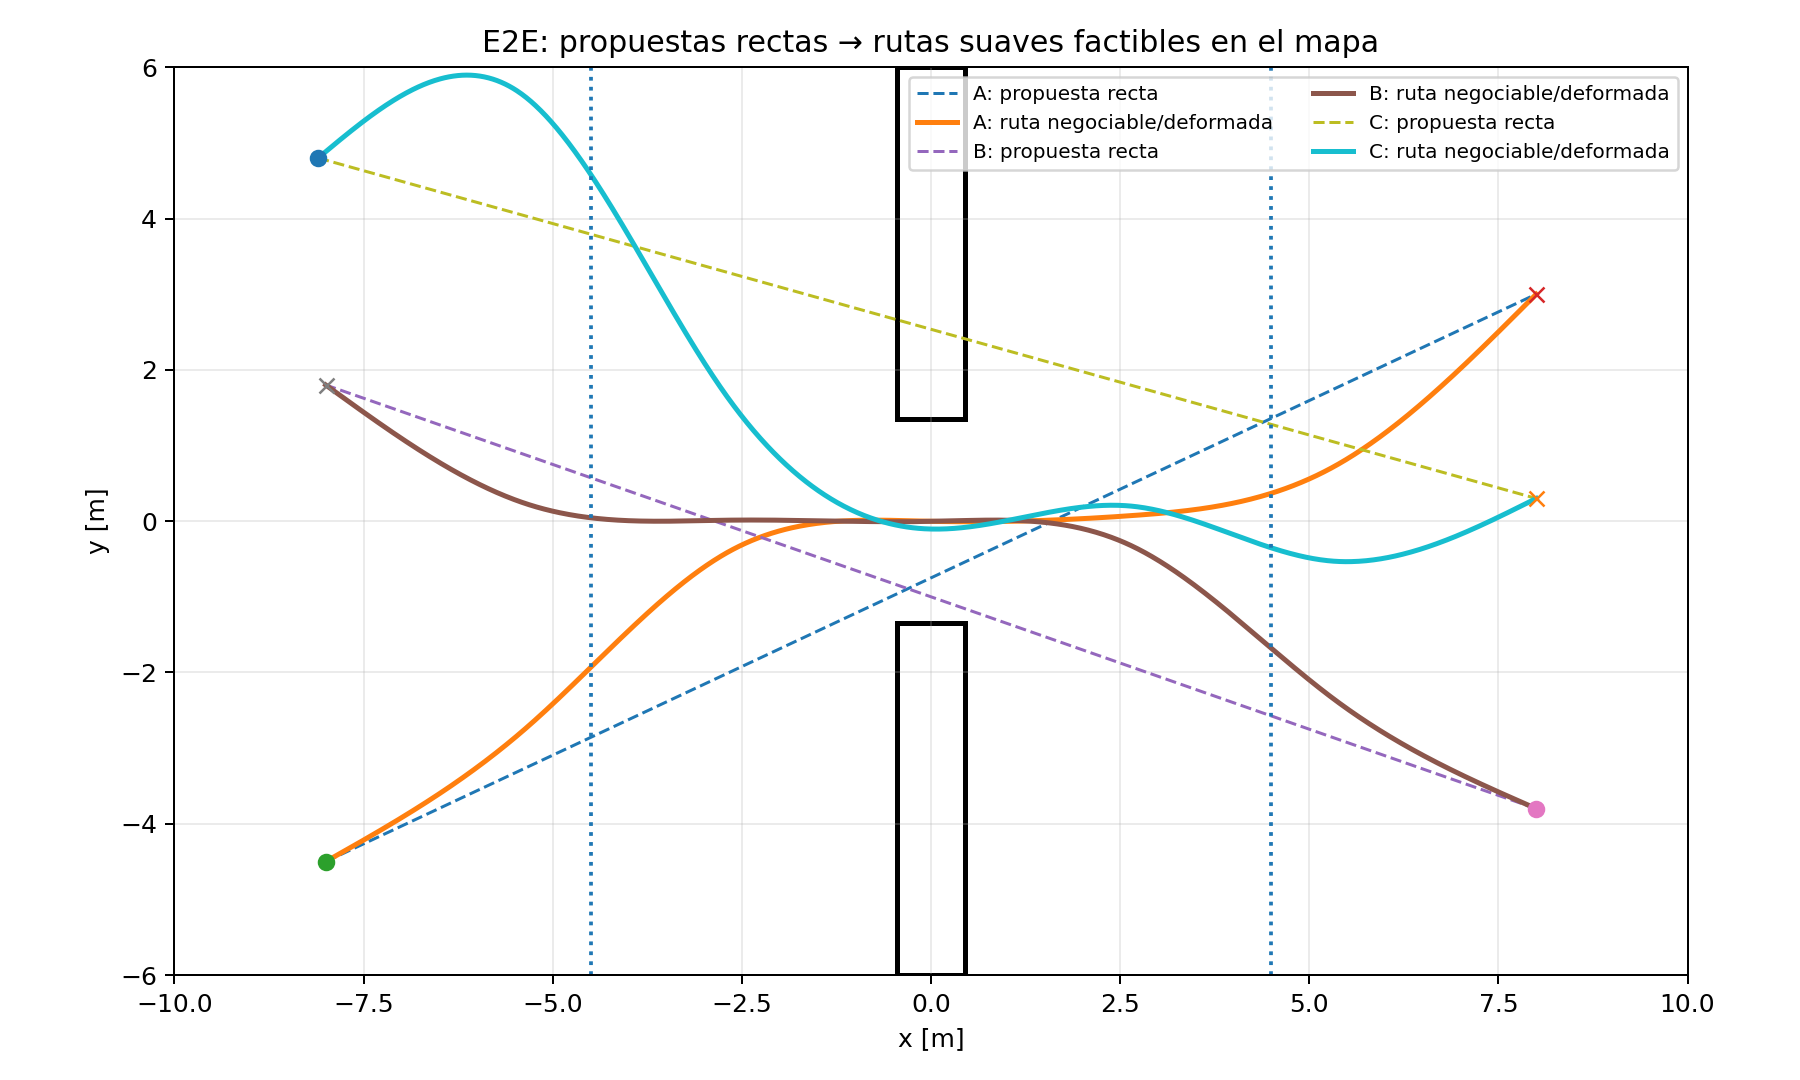
\includegraphics[width=0.82\textwidth]{figures/megajuego/rutas-deformadas.png}
  \caption[Deformación cooperativa de rutas rectas a trayectorias factibles.]{Deformación
  cooperativa de las propuestas rectas iniciales (líneas discontinuas) a
  trayectorias suaves factibles (líneas continuas) que evitan los dos
  obstáculos centrales, para las tres coaliciones del escenario.}
  \label{fig:megajuego-routes}
  \viusource{simulación propia, \texttt{simulate\_e2e\_megagame.py}}
\end{figure}

\begin{figure}[!htbp]
  \centering
  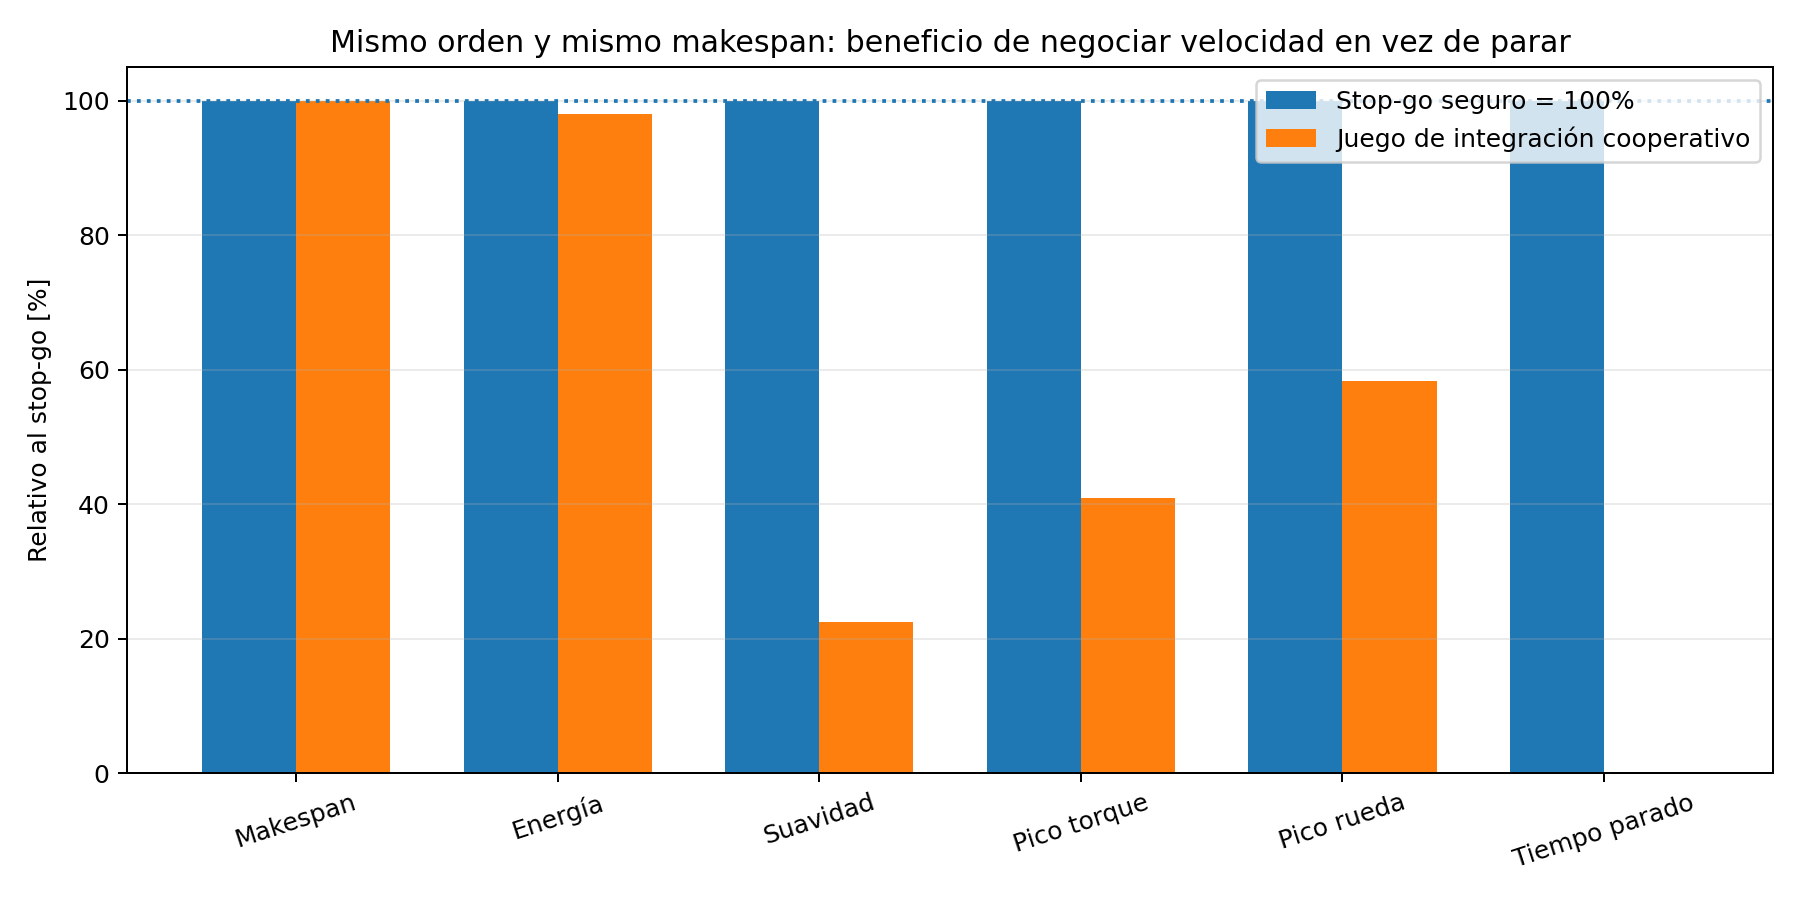
\includegraphics[width=0.82\textwidth]{figures/megajuego/stopgo-vs-cooperativo.png}
  \caption[Ejecución cooperativa frente a parada segura, mismo orden y mismo makespan.]{Ejecución
  cooperativa frente a parada segura (\emph{stop-go}), con idéntico orden y
  makespan. La negociación de velocidad evita las tres paradas del método de
  referencia y reduce energía ($-1.97$\,\%), coste de aceleración
  ($-77.6$\,\%) y torque pico ($-59.1$\,\%).}
  \label{fig:megajuego-stopgo}
  \viusource{simulación propia, \texttt{simulate\_e2e\_megagame.py}}
\end{figure}

La ruta espacial es una solución local del optimizador de \emph{spline} o
potencial. No se certifica su optimalidad global, a diferencia del
reclutamiento y del orden de coaliciones, que sí se comparan contra un oráculo.
El Anexo~\ref{app:reproducibility} registra la ruta del paquete completo, el
\emph{commit} y el entorno.

\zlabel{budget:megajuego-end}
